\documentclass[tikz]{standalone}

\usepackage{amsmath}
\usepackage{circuitikz}

\usetikzlibrary{positioning}

\begin{document}
	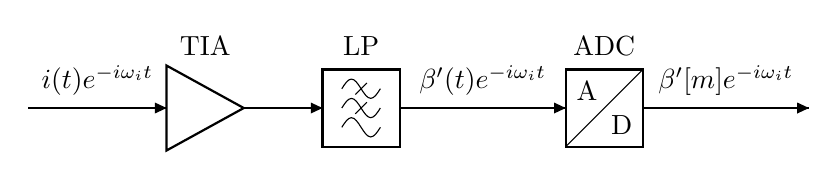
\begin{tikzpicture}
		\coordinate (in) at (0,0);
		\node [ampshape, right=5em of in, label=TIA] (tia) {};
		\node [lowpassshape, right=of tia, label=LP] (lp) {};
		\node [adcshape, right=6em of lp, label=ADC] (adc) {};
		\coordinate [right=6em of adc] (out);

		\draw (in) to[short, l={$i(t)e^{-i\omega_it}$}] (tia.west) node[inputarrow]{};
		\draw (tia.east) -- (lp.west) node[inputarrow]{};
		\draw (lp.east) to[short, l=$\beta^\prime(t)e^{-i\omega_it}$] (adc.west) node[inputarrow]{};
		\draw (adc.east) to[short, l={$\beta^\prime[m]e^{-i\omega_it}$}] (out) node[inputarrow]{};
	\end{tikzpicture}
\end{document}
